
% ----------------------------------------------------------------------
%  Set the document class
% ----------------------------------------------------------------------
\documentclass[11pt,a4paper,twoside]{article}

% ----------------------------------------------------------------------
% Define external packages, language, margins, fonts and new commands
% ----------------------------------------------------------------------
%\input{preamble} 
\usepackage[utf8]{inputenc}   % <<<<< Linux
\usepackage[english]{babel} % <<<<< English
\usepackage{notoccite}
\usepackage[skip=0.5\baselineskip]{caption}
\hyphenation{GTKWave}
\usepackage{listings}
\usepackage[all]{nowidow}

%blind text
\usepackage{lipsum}

\usepackage{graphicx}
\graphicspath{ {./} {../../figlib/} }
\def\FontLn{% 16 pt normal
  \usefont{T1}{phv}{m}{n}\fontsize{16pt}{16pt}\selectfont}
\def\FontLb{% 16 pt bold
  \usefont{T1}{phv}{b}{n}\fontsize{16pt}{16pt}\selectfont}
\def\FontMn{% 14 pt normal
  \usefont{T1}{phv}{m}{n}\fontsize{14pt}{14pt}\selectfont}
\def\FontMb{% 14 pt bold
  \usefont{T1}{phv}{b}{n}\fontsize{14pt}{14pt}\selectfont}
\def\FontSn{% 12 pt normal
  \usefont{T1}{phv}{m}{n}\fontsize{12pt}{12pt}\selectfont}

% Use Arial font as default
%
\renewcommand{\rmdefault}{phv}
\renewcommand{\sfdefault}{phv}
\usepackage{geometry}	
\geometry{verbose,tmargin=2.5cm,bmargin=2.5cm,lmargin=2.5cm,rmargin=2.5cm}

%\usepackage{setspace}
%\renewcommand{\baselinestretch}{1.5}

\usepackage[pdftex]{hyperref} % enhance documents that are to be
                              % output as HTML and PDF
\hypersetup{colorlinks,       % color text of links and anchors,
                              % eliminates borders around links
%            linkcolor=red,    % color for normal internal links
            linkcolor=black,  % color for normal internal links
            anchorcolor=black,% color for anchor text
%            citecolor=green,  % color for bibliographical citations
            citecolor=black,  % color for bibliographical citations
%            filecolor=magenta,% color for URLs which open local files
            filecolor=black,  % color for URLs which open local files
%            menucolor=red,    % color for Acrobat menu items
            menucolor=black,  % color for Acrobat menu items
%            pagecolor=red,    % color for links to other pages
            pagecolor=black,  % color for links to other pages
%            urlcolor=cyan,    % color for linked URLs
            urlcolor=black,   % color for linked URLs
	          bookmarks=true,         % create PDF bookmarks
	          bookmarksopen=false,    % don't expand bookmarks
	          bookmarksnumbered=true, % number bookmarks
	          pdftitle={report},
            pdfauthor={Andre C. Marta},
%            pdfsubject={Thesis Title},
%            pdfkeywords={Thesis Keywords},
            pdfstartview=FitV,
            pdfdisplaydoctitle=true}

\usepackage[numbers,sort&compress]{natbib} % <<<<< References in numbered list [1],[2],...
\usepackage{subcaption} 
\usepackage{mdframed}

%%%%%%%%%%%%%%%%%%%%%%%%%%%%%%%%%%%%%%%%%%%%%%%%%%%%%%%%%%%%%%%%%%%%%%%%
%     Begin Document                                                   %
%%%%%%%%%%%%%%%%%%%%%%%%%%%%%%%%%%%%%%%%%%%%%%%%%%%%%%%%%%%%%%%%%%%%%%%%


\begin{document}

% Set plain page style (no headers, footer with centered page number)
\pagestyle{plain}

% Set roman numbering (i,ii,...) before the start of chapters
%\pagenumbering{roman}

% ----------------------------------------------------------------------
%  Cover page
% ----------------------------------------------------------------------
%%%%%%%%%%%%%%%%%%%%%%%%%%%%%%%%%%%%%%%%%%%%%%%%%%%%%%%%%%%%%%%%%%%%%%%%
%                                                                      %
%     File: Thesis_FrontCover.tex                                      %
%     Tex Master: Thesis.tex                                           %
%                                                                      %
%     Author: Andre C. Marta                                           %
%     Last modified :  2 Jul 2015                                      %
%                                                                      %
%%%%%%%%%%%%%%%%%%%%%%%%%%%%%%%%%%%%%%%%%%%%%%%%%%%%%%%%%%%%%%%%%%%%%%%%

\thispagestyle {empty}

% IST Logo - Signature A
% parameters: bb=llx lly urx ury (bounding box), width=h_length, height=v_length, angle=angle, scale=factor, clip=true/false, draft=true/false. 
\includegraphics[bb=9.5cm 11cm 0cm 0cm,scale=0.29]{IST_A_CMYK_POS}

\begin{center}
%
% Figure (Image or plot)
\vspace{1.0cm}
% height = 50 mm
%\includegraphics[height=50mm]{Figures/Airbus_A350.jpg}

% Title, author and degree
\vspace{1cm}
{\FontLb Circuit Theory and Electronics Fundamentals} \\ % <<<<< EDIT TITLE
\vspace{1cm}
{\FontSn Department of Electrical and Computer Engineering, Técnico, University of Lisbon} \\ % <<<<< EDIT COURSE
\vspace{1cm}
{\FontSn Laboratory Four Report} \\
\vspace{1cm}
{\FontSn Francisco Batista, 95792.} \\
{\FontSn Miguel Jesus, 95833.} \\
{\FontSn Pedro Monteiro, 96465.} \\
\vspace{1cm}
{\FontSn May 23, 2021} \\ % <<<<< EDIT DATE (corresponds to date of oral examination)
%
\end{center}



% ----------------------------------------------------------------------
% Dedication page (optional)
% ----------------------------------------------------------------------
%\input{dedication} 
%\cleardoublepage

% ----------------------------------------------------------------------
%  Acknowledgments (optional)
% ----------------------------------------------------------------------
%\input{acknowledgements}
%\cleardoublepage

% ----------------------------------------------------------------------
%  Abstract (both in English and Portuguese)
% ----------------------------------------------------------------------
%\input{resumo} 
%\cleardoublepage

%\input{abstract} 

% ----------------------------------------------------------------------
%  Table of contents, list of tables, list of figures and nomenclature
% ----------------------------------------------------------------------

% Table of contents

\vspace{8.5cm}

\tableofcontents

% List of tables
%\addcontentsline{toc}{section}{\listtablename}
%\listoftables
%\cleardoublepage 

% List of figures
%\addcontentsline{toc}{section}{\listfigurename}
%\listoffigures
%\cleardoublepage 

% Set arabic numbering (1,2,...) after preface
%
%\setcounter{page}{1}
%\pagenumbering{arabic}

% ----------------------------------------------------------------------
%  Body
% ----------------------------------------------------------------------


\section{Introduction}
\label{Introduction}

\par The main goal of this laboratory assignment is to design a circuit of an audio amplifier and to analyse it theoretically, as well as simulating it using Ngspice.
\par To successfully create this circuit we had to architecture the gain stage and the output stage
\par We were also asked to analyse quantitatively the quality of the designed circuit using the Merit expression presented bellow. 

\begin {equation}
	Merit = \frac{VoltageGain*bandwidth}{Cost*CutoffFreq}
	\label{costofmerit}
\end{equation}


\section{Simulation Analysis}
\label{sec:simulation}

Before proceeding the theoretycal analysis, we simulated the circuit via the Ngspice software in order to perfect our parameters` values.

\begin{table}[h]
  \centering
  \begin{tabular}{|l|r|}
    \hline    
    {\bf Parameters} & {\bf Values} \\ \hline
    \input{op_TAB3}
  \end{tabular}
  \caption{Parameters` values.}
  \label{tab:s01}
\end{table}

To simulate the transistor behaviour, we utilized the NPN and the PNP models provided by the professor.

We performed transient and frequency analysis of the combined gain and output stages, that represent, respectively, the common emitter and collector amplifiers.

\begin{figure}[h] \centering
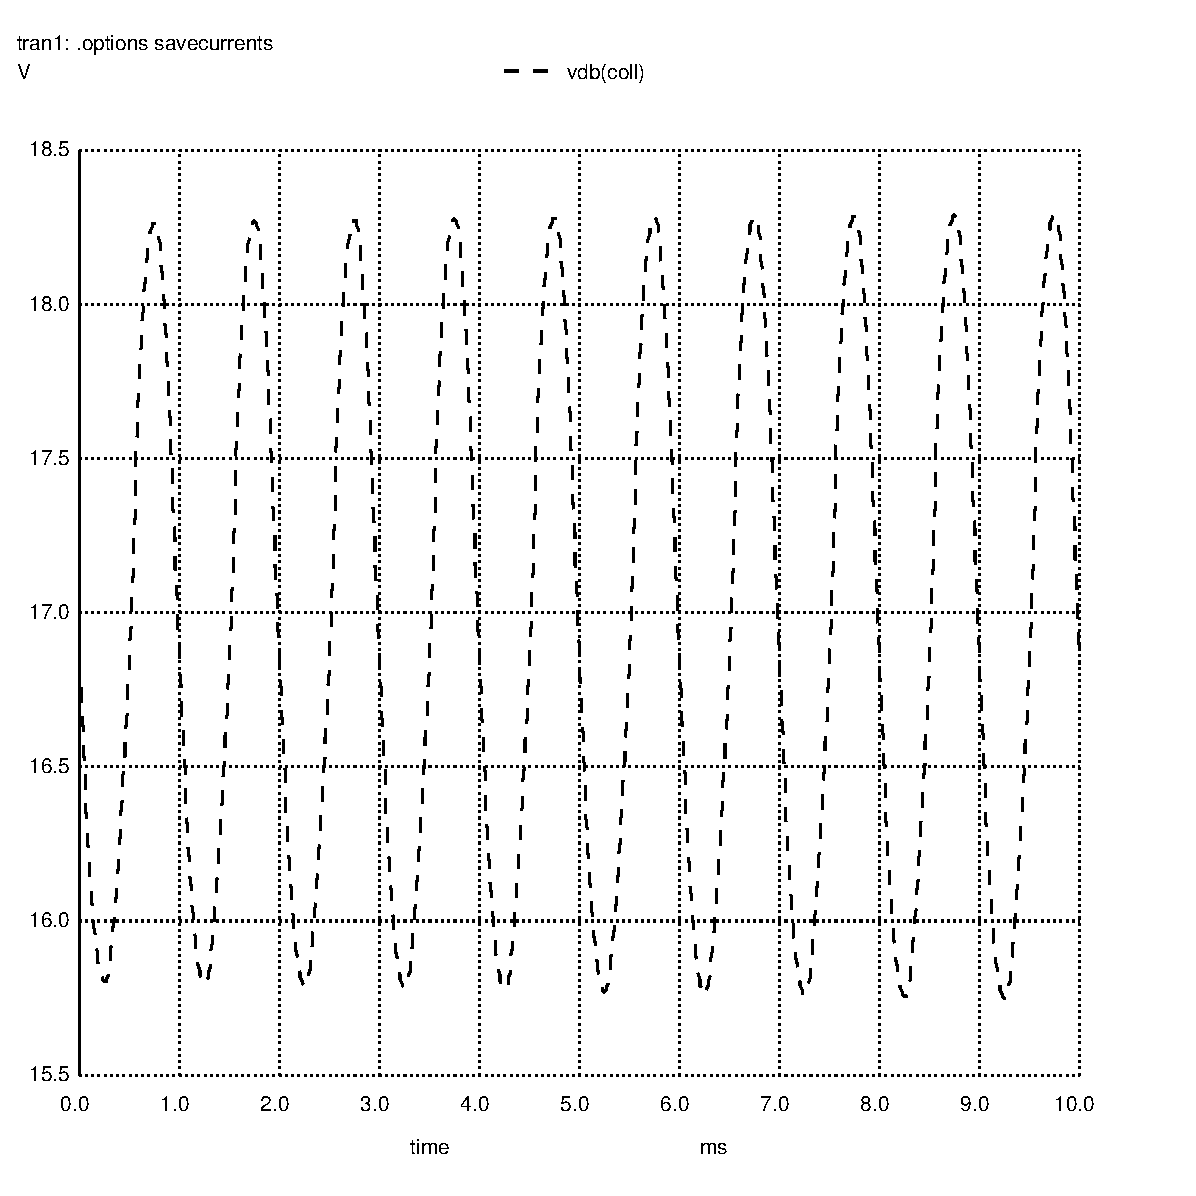
\includegraphics[width=0.5\linewidth]{vo1.eps}
\caption{Voltage in the collector, transient analysis.}
\label{fig:s1}
\end{figure}


\begin{figure}[h] \centering
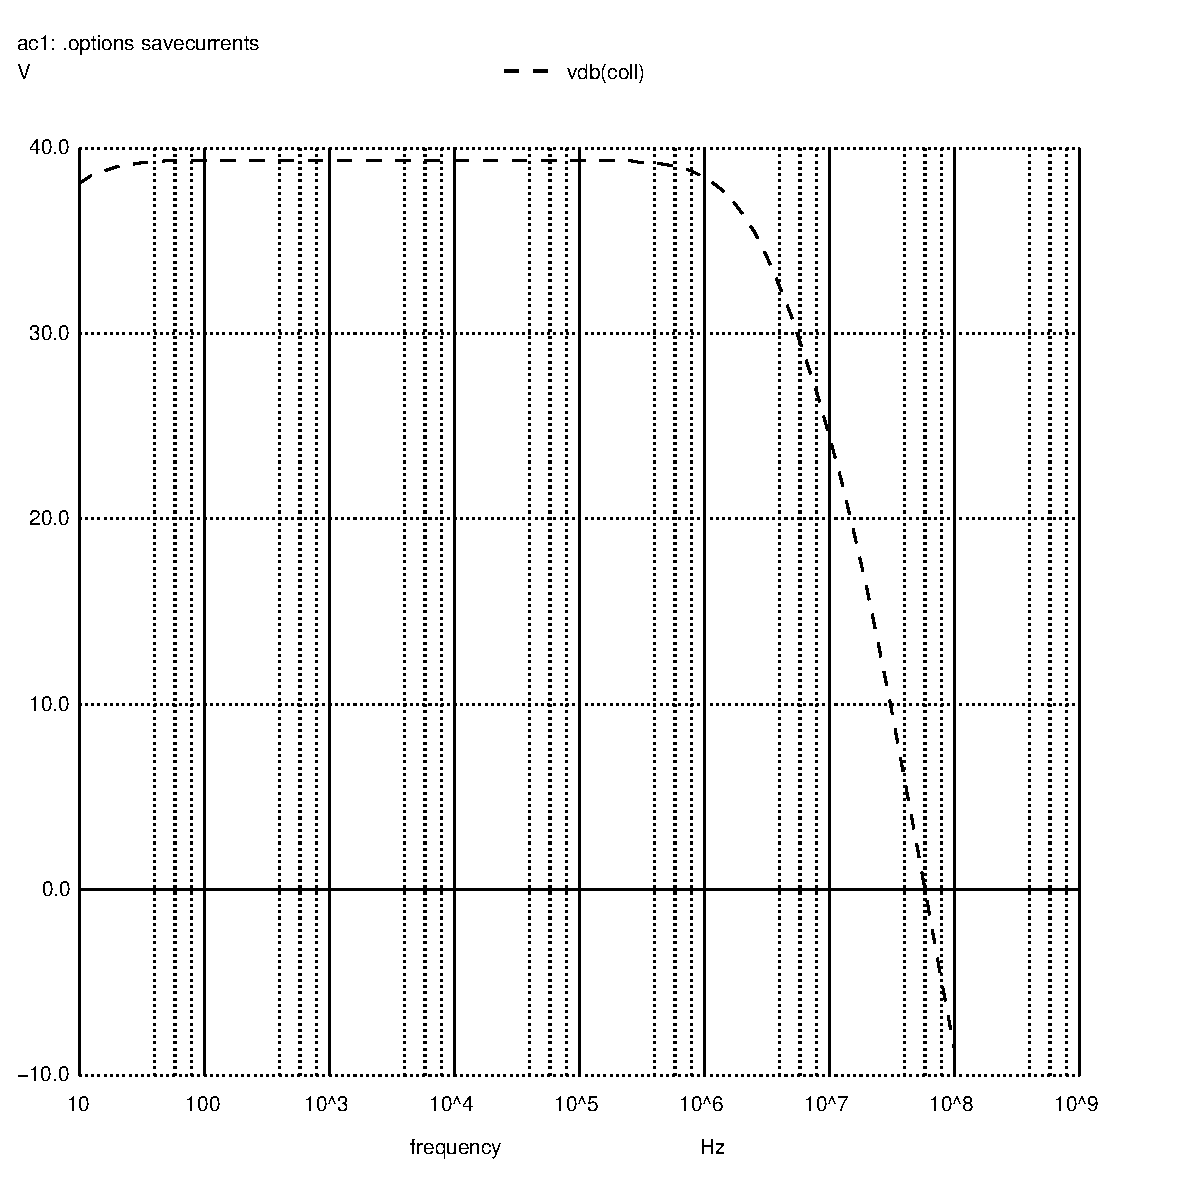
\includegraphics[width=0.5\linewidth]{vo1f.eps}
\caption{Voltage in the collector[dB], frequency analysis.}
\label{fig:s2}
\end{figure}



\begin{figure}[h] \centering
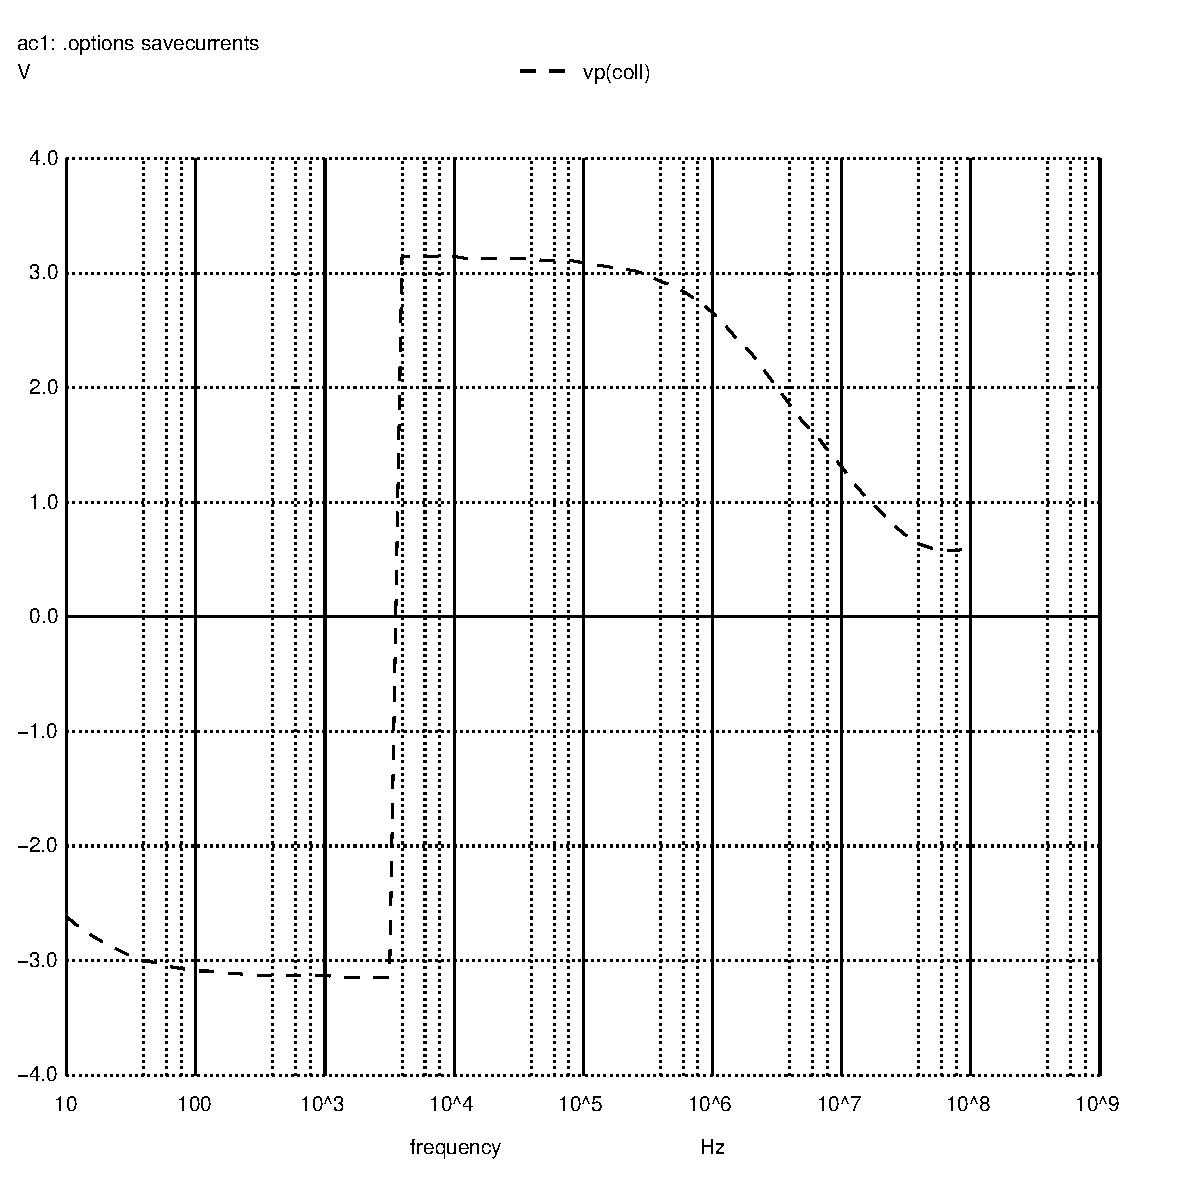
\includegraphics[width=0.5\linewidth]{vo3f.eps}
\caption{Phase voltage in the collector, frequency analysis.}
\label{fig:s3}
\end{figure}

\vspace{10.0cm}


\begin{figure}[h] \centering
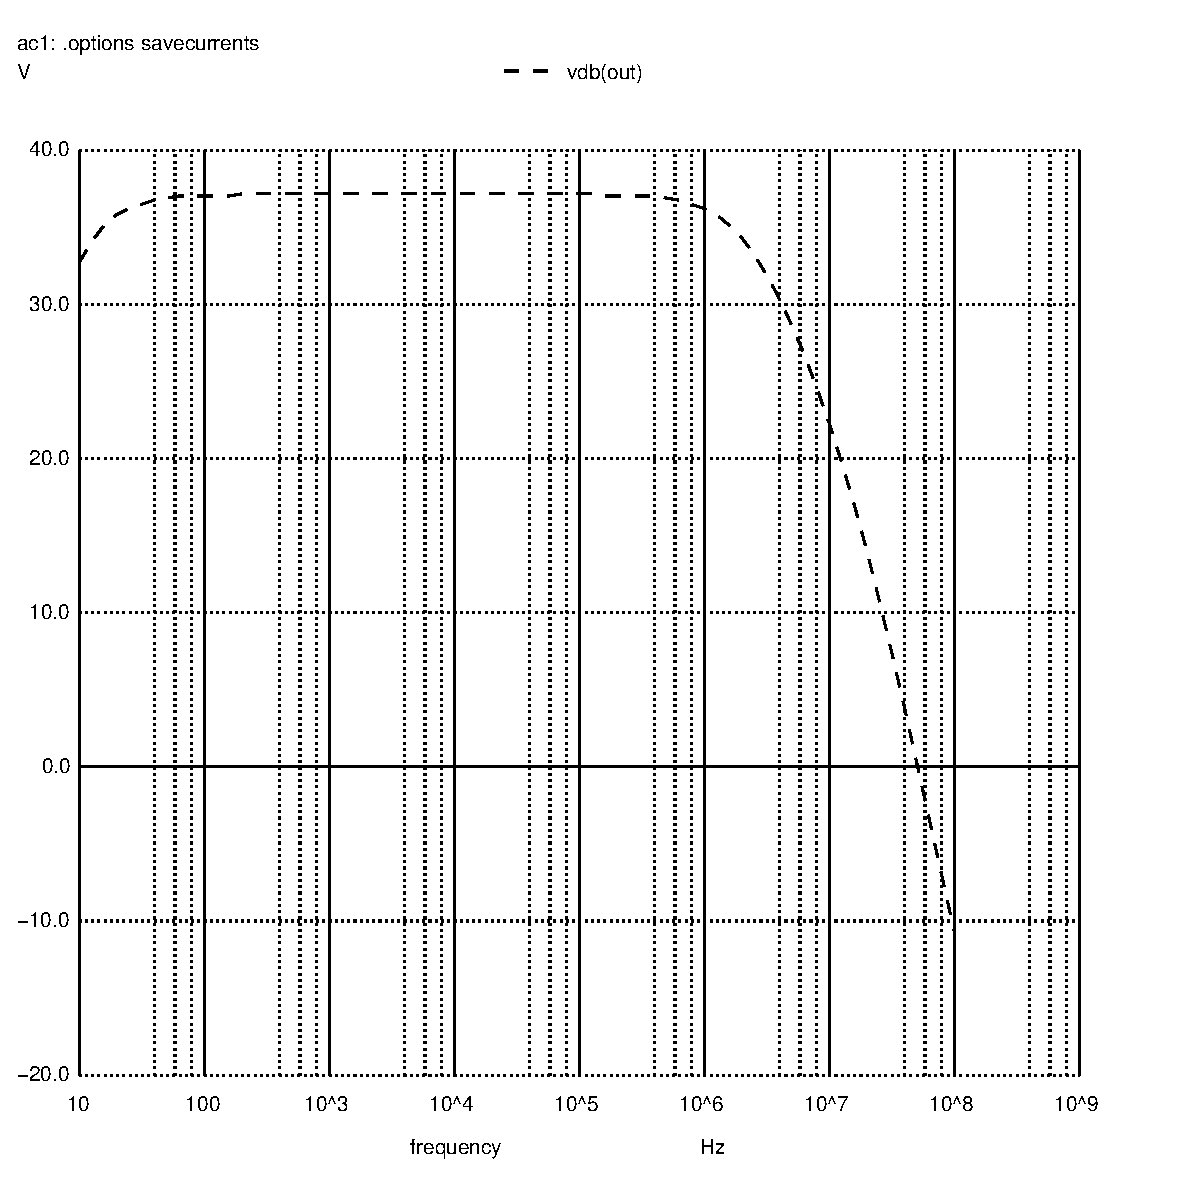
\includegraphics[width=0.5\linewidth]{vo2f.eps}
\caption{Output voltage[dB].}
\label{fig:s4}
\end{figure}

\vspace{10.0cm}

\begin{figure}[h] \centering
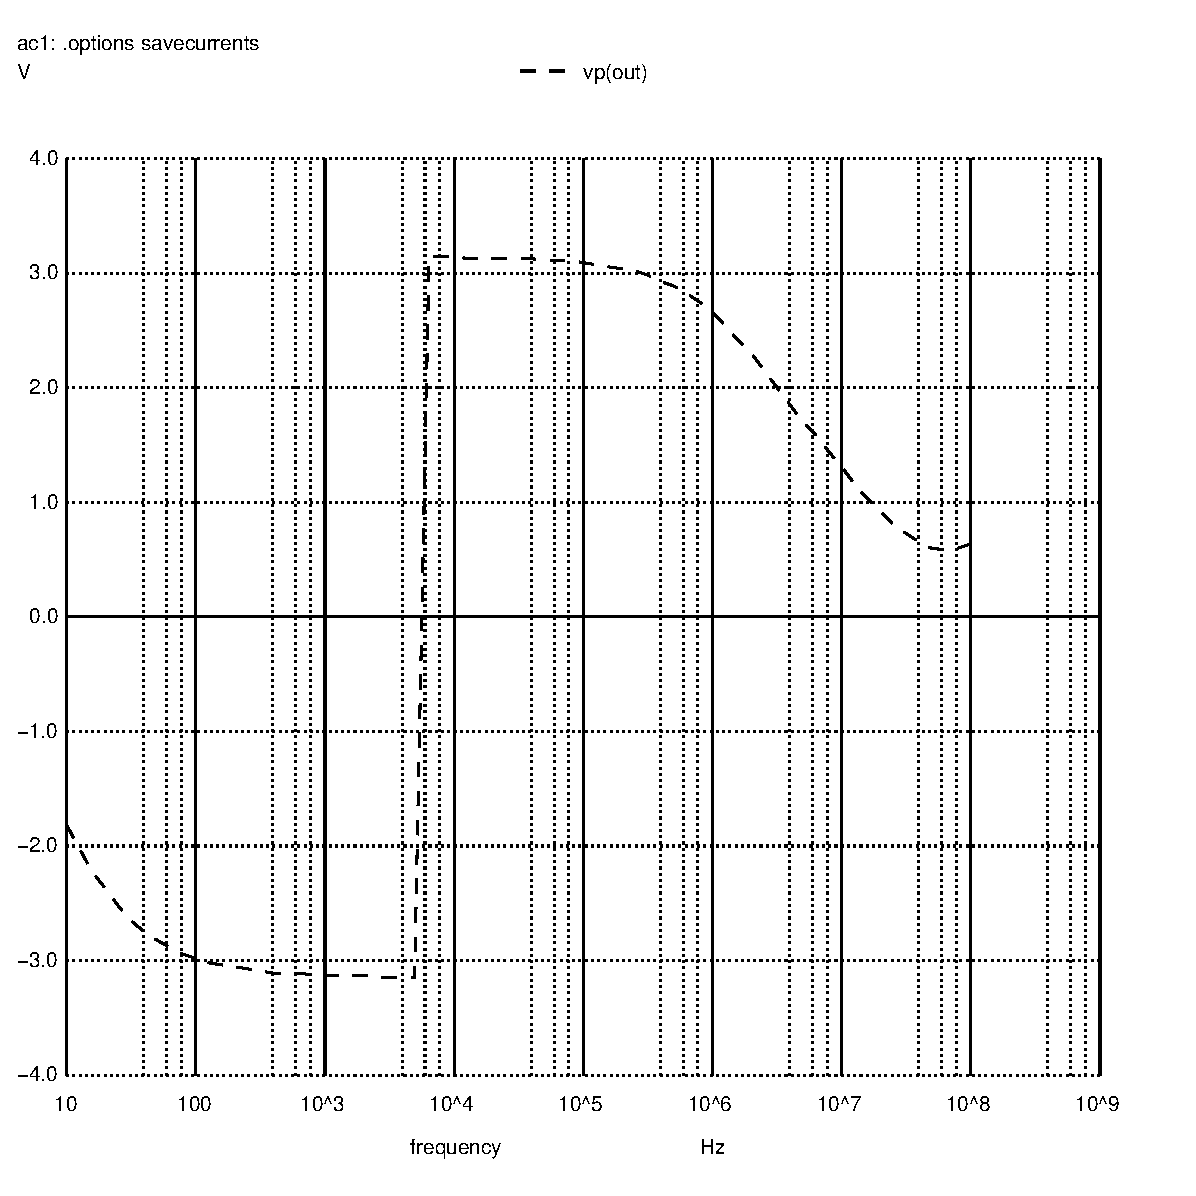
\includegraphics[width=0.5\linewidth]{vo4f.eps}
\caption{Output voltage phase.}
\label{fig:s5}
\end{figure}

\vspace{10.0cm}

From the simulation we were able to compute the important values of the cut-off frequencies, the gain and the bandwidth, which allowed us to calculate our merit. Furthermore, we found the values for the input and output impedances.

\begin{table}[h]
  \centering
  \begin{tabular}{|l|r|}
    \hline    
    {\bf Parameters} & {\bf Values} \\ \hline
    \input{op_TAB}
  \end{tabular}
  \caption{Values computed in the simulation.}
  \label{tab:s1}
\end{table}

\begin{table}[h]
  \centering
  \begin{tabular}{|l|r|}
    \hline    
    {\bf Parameters} & {\bf Values} \\ \hline
    \input{op_TAB2}
  \end{tabular}
  \caption{Output impedance.}
  \label{tab:s2}
\end{table}




\section{Theoretical Analysis}
\label{sec:analysis}

\par In this section, we used the theorectical model as presented in the lectures. To do so we adopted the equations provided in lecture 16 and 17 and utilised the values of the circuit parameters, that we optimized with the help of Ngspice tool, as showcased previously.

\par The circuit was divided in two main parts, the gain and output stages. These were combined together because they complemented one another.

\par The gain stage which consists of a common emitter amplifier has the advantage of generating a high, desirable gain. However, along with this comes the cost of having a very high output impedance which squanders the gain.

\begin{table}[h]
  \centering
  \begin{tabular}{|l|r|}
    \hline    
    {\bf Parameters} & {\bf Values} \\ \hline
    |VT| & 0.025000 \\ \hline
|beta| & 178.700000 \\ \hline
|VA| & 69.700000 \\ \hline
|VBEON| & 0.700000 \\ \hline
|Vcc| & 12.000000 \\ \hline
|Req| & 8461.538462 \\ \hline
|Veq| & 1.846154 \\ \hline
|IB1| & 0.000026 \\ \hline
|IC1| & 0.004613 \\ \hline
|IE1| & 0.004639 \\ \hline
 |$V_{emit}$| & 0.927733 \\ \hline
|$V_{coll}$| & 6.925864  \\ \hline
|VCE| & 5.998131 \\ \hline|$V_{base}$| & 1.627733  \\ \hline
  \end{tabular}
  \caption{Transistor`s parameters.}
  \label{tab:1}
\end{table}

\begin{table}[h]
  \centering
  \begin{tabular}{|l|r|}
    \hline    
    {\bf Parameters} & {\bf Values} \\ \hline
    |gm1| & 0.184514 \\ \hline
|ro1| & 15109.960453 \\ \hline
|rpi| & 968.489933 \\ \hline
  \end{tabular}
  \caption{Parameters of slide 10, lecture 16.}
  \label{tab:2}
\end{table}

\begin{table}[h]
  \centering
  \begin{tabular}{|l|r|}
    \hline    
    {\bf Parameters} & {\bf Values} \\ \hline
    |Input impedance| & 869.023345 \\ \hline
|Output impedance| & 1025.354537 \\ \hline
|Gain| & 169.668298 \\ \hline
|Gain(dB)| & 44.592014 \\ \hline
  \end{tabular}
  \caption{Gain and impedances.}
  \label{tab:3}
\end{table}


\par In order to reduce the high impedance value that is associated with the gain stage, we developed an output stage that allows to rectify the problem we had previously. Once again, we followed the instructions given in the lectures.

\begin{table}[h]
  \centering
  \begin{tabular}{|l|r|}
    \hline    
    {\bf Parameters} & {\bf Values} \\ \hline
    |VO2| & 7.625864 \\ \hline
|$V_{coll}$| & 6.925864 \\ \hline
|VA| & 7.625864 \\ \hline
|$V_{emit}$| & 12.000000 \\ \hline
|Vcc| & 0.000087 \\ \hline
|IB2| & 0.019795 \\ \hline
|IC2| & 0.019882 \\ \hline
|IE2| & 
  \end{tabular}
  \caption{Parameter values for the output stage.}
  \label{tab:4}
\end{table}


\begin{table}[h]
  \centering
  \begin{tabular}{|l|r|}
    \hline    
    {\bf Parameters} & {\bf Values} \\ \hline
    |gm2| & 0.791814 \\ \hline
|go2| & 0.000532 \\ \hline
|gpi2| & 0.003484 \\ \hline
|ge2| & 0.004545 \\ \hline
|Input Impedance| & 26837.230759 \\ \hline
|Output Impedance| & 1.249414 \\ \hline
|Gain| & 0.989304 \\ \hline
|Gain(dB)| & -0.093408 \\ \hline
  \end{tabular}
  \caption{Output stage impedance and gain.}
  \label{tab:5}
\end{table}

\vspace{100.0cm}

\par Finally, the gain results of the total circuit.

\begin{figure}[h] \centering
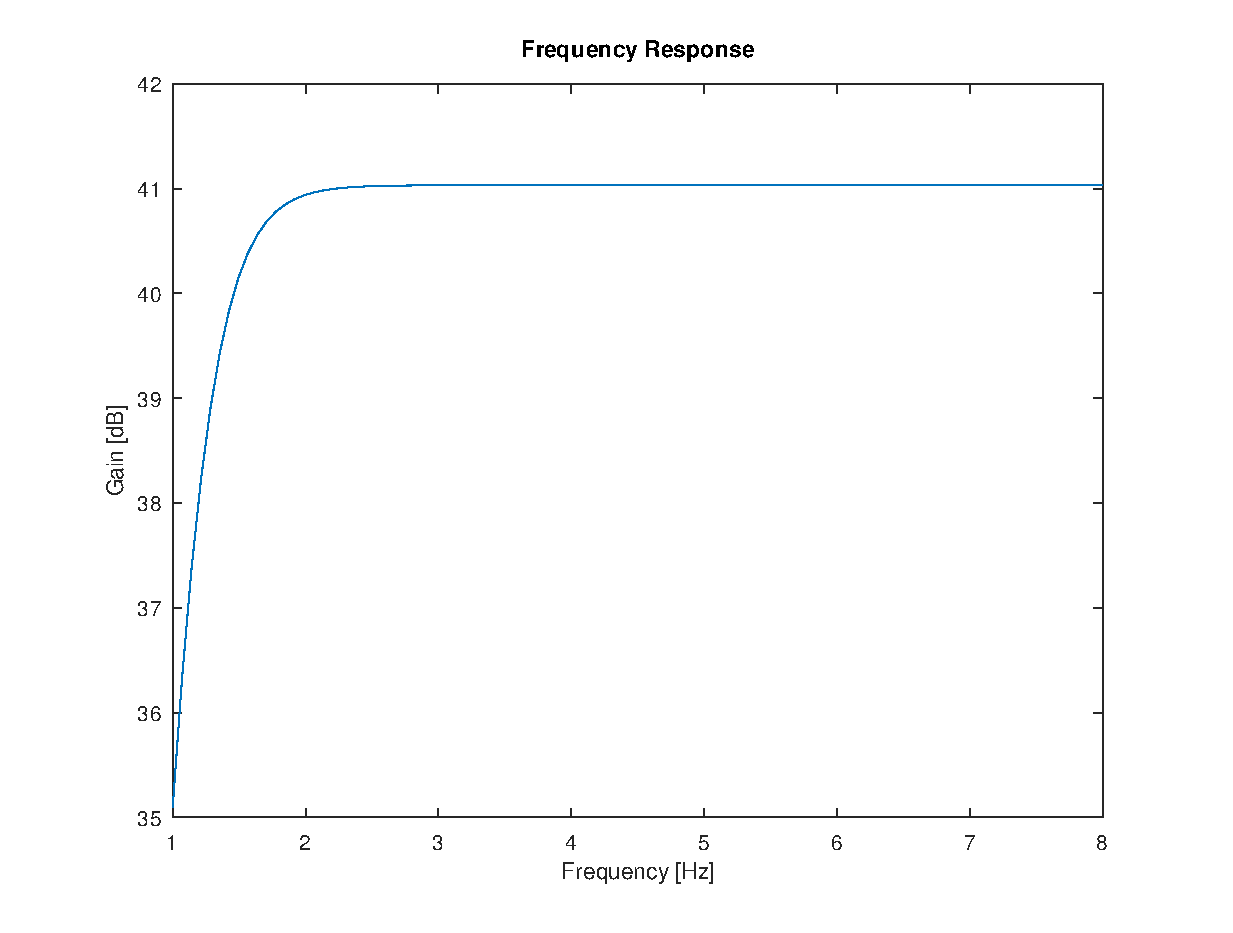
\includegraphics[width=0.6\linewidth]{freqresponse.eps}
\caption{Plot of Gain in order of the Frequency (Hz).}
\label{fig:plotA1}
\end{figure}


\newpage

\section{Conclusion}
\label{sec:conclusion}

To sum up, in this assignment, the main goal was 


%\cleardoublepage

% ----------------------------------------------------------------------
%  Bibliography
% ----------------------------------------------------------------------
%\addcontentsline{toc}{section}{\bibname}
%\bibliographystyle{abbrvunsrtnat} % <<<<< SELECT IF USING REFERENCES BY NUMBER (CITATION ORDER)
%\bibliography{../../../BIBfile.bib}

% ----------------------------------------------------------------------
\end{document}
% ----------------------------------------------------------------------

